
%(BEGIN_QUESTION)
% Copyright 2009, Tony R. Kuphaldt, released under the Creative Commons Attribution License (v 1.0)
% This means you may do almost anything with this work of mine, so long as you give me proper credit

Read and outline the ``Compensated Leg Systems'' subsection of the ``Hydrostatic Pressure'' section of the ``Continuous Level Measurement'' chapter in your {\it Lessons In Industrial Instrumentation} textbook.  Note the page numbers where important illustrations, photographs, equations, tables, and other relevant details are found.  Prepare to thoughtfully discuss with your instructor and classmates the concepts and examples explored in this reading.

\underbar{file i03951}
%(END_QUESTION)





%(BEGIN_ANSWER)


%(END_ANSWER)





%(BEGIN_NOTES)

If a vessel is unvented, any gas pressure above the liquid will become added to the liquid's hydrostatic pressure to skew the pressure sensed at the bottom.  If we are trying to measure liquid level via hydrostatic pressure, the gas pressure effect will mess it up.

A differential pressure sensor, however, gives us a way to compensate for gas pressure inside a sealed vessel: connect the other port of the transmitter to a ``compensating leg'' running to the top of the vessel, so that the transmitter only senses the difference in pressure between bottom and top, thus canceling out any gas pressure from the measurement.  Differential pressure at the instrument will now be equal to hydrostatic pressure (only).

\vskip 10pt

If condensible vapors cause the compensating leg to fill with liquid, a constant zero shift will result.  This is called a ``wet leg'' system.  We may guarantee the density of the liquid in the wet leg by either filling it with our own fill fluid, or by using a remote seal.  If the wet leg is always filled with condensed process vapors, a {\it seal pot} may be used to help maintain a nearly constant wet leg head even after bleeding some wet leg liquid out during routine instrument maintenance.  Seal pots are common on steam drum level measurement systems.

\vskip 10pt

As compensating legs are usually taller than the measurement range within the vessel, it is common for the wet leg to exert more hydrostatic pressure than the vessel liquid.  Since many legacy DP transmitters could not handle negative differential pressures, wet leg DP instruments have traditionally been installed with the ``H'' port connected to the wet leg and the ``L'' port connected to the bottom of the vessel.  Even though modern electronic DP transmitters can handle negative differential pressures just fine, we often find them installed the same way (with the ``L'' port connected to the vessel bottom) out of habit.  If connected in this manner, be aware that the action of the transmitter will be reverse: more liquid level results in less output signal.








\vskip 20pt \vbox{\hrule \hbox{\strut \vrule{} {\bf Suggestions for Socratic discussion} \vrule} \hrule}

\begin{itemize}
\item{} A helpful ``active reading'' technique for technical texts is to work through every mathematical example presented, to ensure you understand the math as you read along.  Apply this technique here, demonstrating how to work through at least one of the calculation examples presented in the textbook.
\item{} Explain why compensating legs must be used in hydrostatic level measurement applications when the process vessel is not vented.
\item{} In a compensated-leg system where the DP transmitter uses two remote seals, does the height of the transmitter relative to the process connection points matter?  In other words, can we elevate or suppress this DP transmitter without changing its LRV and URV points?  Explain why or why not.
\item{} In a compensated-leg system where the compensating leg is ``wet'' with some liquid other than the process liquid, does the height of the DP transmitter relative to the process connection points matter?  In other words, can we elevate or suppress this DP transmitter without changing its LRV and URV points?  Explain why or why not.
\item{} Should a DP transmitter equipped with remote seals also be equipped with a three-valve manifold?  Explain why or why not.
\item{} Explain the function of a {\it seal pot} in a compensated-leg system.
\item{} Explain why some DP transmitters used in wet-leg systems are installed ``backwards'' (the H side toward the process vessel and the L side toward the wet leg).
\end{itemize}











\vfil \eject

\noindent
{\bf Summary Quiz:}

Calculate the amount of pressure sensed by the DP transmitter when the process vessel is completely empty (no liquid inside), assuming a specific gravity of the remote seal fill fluid equal to 2.0 (twice as dense as water):

$$\includegraphics[width=15.5cm]{i03951x01.eps}$$

\begin{itemize}
\item{} -480 inches H$_{2}$O 
\vskip 5pt 
\item{} -384 inches H$_{2}$O
\vskip 5pt 
\item{} +96 inches H$_{2}$O
\vskip 5pt 
\item{} -192 inches H$_{2}$O
\vskip 5pt 
\item{} -576 inches H$_{2}$O
\vskip 5pt 
\item{} +240 inches H$_{2}$O 
\end{itemize}

%INDEX% Reading assignment: Lessons In Industrial Instrumentation, Continuous Level Measurement (hydrostatic pressure -- compensated legs)

%(END_NOTES)


